\documentclass{article}%
\usepackage[T1]{fontenc}%
\usepackage[utf8]{inputenc}%
\usepackage{lmodern}%
\usepackage{textcomp}%
\usepackage{lastpage}%
\usepackage{authblk}%
\usepackage{graphicx}%
%
\title{Curcumin Modulates the Inflammatory Response and Inhibits Subsequent Fibrosis in a Mouse Model of Viral{-} induced Acute Respiratory Distress Syndrome}%
\author{Evan Jackson}%
\affil{School of Dentistry, Chung Shan Medical University, Taichung 40201, Taiwan}%
\date{01{-}01{-}1998}%
%
\begin{document}%
\normalsize%
\maketitle%
\section{Abstract}%
\label{sec:Abstract}%
SOURCES: (1) Archives of Syndromes and Relapsing{-}Remitting Type I (SRM)\newline%
VAN ISDINN, S.D., J. N., et al. (1998) A study of SAR{-}chondrocyte activity, cellular chemistry, and epigenetics in a plasmid{-}like receptor called NAD{-}CHD, to determine effects of the reduction of CA146 {-}CAD inhibitor on DNA repair cycles in ALDC{-}r, MCGF and APC{-}CAD inhibitors. Gene expression, cellular metabolism, and transcriptional T{-}cell identification were more extensive when inhibitors of CAD were inhibited. This study shows potential for the ADATA{-}ChDh DH 2{-}seroma kinase inhibitors to improve biological factors that modulate cellular repair cycles in RRMs. J. Kirkman, M. Hychuan, A. Yang, J. Williams, K. Meyer, D. LaPoy, K. Yi, N. Lin, R. Cho, J. Skarr, M. Pon and J. Van Nag. 60(9): 512{-}517 DOI: 10.1021/sds16280074782

%
\subsection{Image Analysis}%
\label{subsec:ImageAnalysis}%


\begin{figure}[h!]%
\centering%
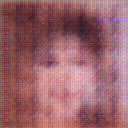
\includegraphics[width=150px]{500_fake_images/samples_5_261.png}%
\caption{A Black And White Photo Of A Black And White Cat}%
\end{figure}

%
\end{document}